\section{Differentiation}

  \begin{definition}[Divided Difference, Average Value]
    Let $f$ be integrable over closed and bounded $[a, b]$. Extend $f$ to take value $f(b)$ on $(b, b +1]$. For $0 < h \leq 1$, we define 
    \begin{enumerate}
      \item the \textbf{divided difference function} as 
        \begin{equation}
          \Diff_h f \coloneqq \frac{f(x + h) - f(x)}{h}
        \end{equation} 
        
      \item the \textbf{average value function} as 
        \begin{equation}
          \Av_h f(x) \coloneqq \frac{1}{h} \int_x^{x + h} f(x)
        \end{equation}
    \end{enumerate}
  \end{definition} 

  Note this important property, which we can think of as a finite version of the fundamental theorem of calculus. 

  \begin{lemma}[Finite Version of Fundamental Theorem of Calculus][thm:Change of Variable]
    We first establish that given integrable $f$ over closed, bounded interval $[a, b]$, we extend $f$ to equal $f(b)$ on $(b, b +1]$. Then for $0 < h \leq 1$, define 
    \begin{equation}
      \Diff_h f \coloneqq \frac{f(x + h) - f(x)}{h}, \qquad \Av_h f(x) \coloneqq \frac{1}{h} \int_{x}^{x + h} f(x)
    \end{equation}
    Then, for all $a \leq u < v \leq b$, 
    \begin{equation}
      \int_u^v \Diff_h f = \Av_h f(v) - \Av_h f(u)
    \end{equation}
  \end{lemma}
  \begin{proof}
    We see by employing a change of basis and the integral properties, 
    \begin{align}
      \int_a^b \Diff_h f & = \int_u^v \frac{f(x + h) - f(x)}{h} \\ 
                         & \frac{1}{h} \int_u^v f(x + h) - \frac{1}{h} \int_u^v f(x) \\ 
                         & = \frac{1}{h} \int_{u+h}^{v+h} f(x) -  \frac{1}{h} \int_u^v f(x) \\ 
                         & = \frac{1}{h} \int_{u+h}^{v} f(x) + \frac{1}{h} \int_{v}^{v+h} f(x) -  \frac{1}{h} \int_u^{u+h} f(x) - \frac{1}{h} \int_{u+h}^v f(x) \\ 
                         & = \frac{1}{h} \int_{v}^{v+h} f(x) -  \frac{1}{h} \int_u^{u+h} f(x) \\ 
                         & = \Av_h f(v) - \Av_h f(u)
    \end{align}
  \end{proof}

  Now, we will establish differentiation and culminate in the fundamental theorem of calculus. 
  We first focus on monotone functions, which has two nice properties. First, they can be discontinuous on at most a countable set, and second, they are differentiable a.e.!\footnote{Note that we gained differentiability by strengthening our assumption for a countable set to a measure 0 set.} Therefore, the \textit{difference} of two increasing functions in an open interval is also differentiable a.e. The class of functions of bounded variation are such functions that can be decomposed as this difference, and we call this the Jordan decomposition. 

  Note that the finite version of the fundamental theorem of calculus applies for integrable functions. We would like a formula that looks more like 
  \begin{equation}
    \int_a^b f^\prime (x) = f(b) - f(a)
  \end{equation}
  In order to do this, we first have to define the derivative. 

  \begin{definition}[Derivative]
    For function $f: E \subset \mathbb{R} \to \mathbb{R}$ and an interior point $x \in E^\circ$, we define the \textbf{upper and lower derivatives} as 
    \begin{equation}
      \overline{D} f(x) \coloneqq \lim_{h \to 0} \sup_{0 < |t| < h} \frac{f(x + t) - f(x)}{t}, \qquad \underline{D} f(x) \coloneqq \lim_{h \to 0} \inf_{0 < |t| < h} \frac{f(x + t) - f(x)}{t}
    \end{equation}
    If $\overline{D} f (x) = \underline{D} f (x) < +\infty$, then this value is the \textbf{derivative} of $f$ at $x$, denoted $f^\prime (x)$, and we say that $f$ is \textbf{differentiable} at $x$. 
  \end{definition} 

  So given the punctured neighborhood $(x - h, x + h) \setminus \{x\}$, you can think of the upper derivative as the ``maximum slope,'' and the lower derivative as the ``minimum slope.''\footnote{Kiselev told me that while he always thinks of integrals as Lebesgue integrals, he often just thinks of the derivative as the limit rather than the limit of supremums/infimums.}

  Note that as $h$ goes to $0$, the first is nondecreasing and the second is nonincreasing, and clearly 
  \begin{equation}
    \underline{D} f(x) \leq \overline{D} f(x)
  \end{equation}
 
  \begin{example}[Derivative of Riemann Function]
    Consider the Riemann function $\chi_\mathbb{Q}$. Then 
    \begin{enumerate}
      \item To compute the upper derivative, consider when $x$ is a rational. Then no matter how small we set $h$, there will always be a rational and an irrational in $(x - h, x + h) \setminus \{x\}$. 
        \begin{equation}
          \overline{D} \chi_{\mathbb{Q}} = \begin{cases} 
            0 & \text{ if } x \in \mathbb{Q} \\ 
            +\infty & \text{ if } x \in \mathbb{Q}^c
          \end{cases} 
        \end{equation}

      \item To compute the lower derivative, consider when $x$ is a rational. Then no matter how small we set $h$, there will always be a rational and an irrational in $(x - h, x + h) \setminus \{x\}$. 
        \begin{equation}
          \overline{D} \chi_{\mathbb{Q}} = \begin{cases} 
            -\infty & \text{ if } x \in \mathbb{Q} \\ 
            0 & \text{ if } x \in \mathbb{Q}^c
          \end{cases} 
        \end{equation}
    \end{enumerate}
  \end{example}

  Great, so we have defined the derivative, and now we want to try and show something like 
  \begin{equation}
    \lim_{h \to 0^+} \int_a^b \Diff_h f = \lim_{h \to 0^+} \Av_h f(b) - \Av_h f(a)
  \end{equation}
  If $f$ is continuous, then we can show that the RHS is $f(b) - f(a)$. If $f$ is absolutely continuous, then we can show that the LHS becomes $\int_a^b f^\prime$. 

\subsection{Monotone Functions}

  Monotone functions are a nice class of functions to study for differentiation and for constructing more general measures. 

  \begin{theorem}[Monotone Functions has At Most Countable Discontinuities]
    Suppose $f$ is monotone, increasing on $[a, b]$. Then, the set of discontinuities of $f$ at most countable. 
  \end{theorem}
  \begin{proof}
    The idea is to show that the one-sided limits must exist by monotonicity, and one this is true, we can create intervals in the codomain for which there is a jump. Let $x_k$ be any point of discontinuity. Note that 
    \begin{align}
      \lim_{x \to x_k^-} f(x) & \coloneqq \sup \{ f(x) \mid a < x < x_k \} \\
      \lim_{x \to x_k^+} f(x) & \coloneqq \inf \{ f(x) \mid x_k < x < b \} 
    \end{align}
    both exist by monotonicity, but since there is a discontinuity, we have 
    \begin{equation}
      L_k^- = \lim_{x \to x_k^-} f(x) < \lim_{x \to x_k^+} f(x) = L_k^+
    \end{equation}
    Then, $L_k^+ - L_k^-$ is a jump of $f$ at $x_k$. These intervals $[L_k^-, L_k^+]$ are disjoint due to monotonicity, and each interval contains a rational number. So there can only be at most countable intervals.\footnote{We can detour to a slight generalization for not necessarily monotone functions. Recall that a point $x$ is a discontinuity of the first kind of $f(x)$ if both one-sided limits exist. Then, the set of discontinuities of the first kind is countable. Idea of the proof. Look at some jump discontinuity and record the jump $\eta > 0$. Then, find $\delta > 0$ s.t. if $0 < y - x < \delta$, then $\big| f(x)  - \lim_{y \to x^+} f(y) \big|  < \frac{\eta}{10}$. Then look at the rectangle on the graph associated with each jump. Because the limits exist, you can pick the rectangles so small that they are completely disjoint. Look at picture. }
  \end{proof}

  The following is a sort-of reverse statement.  

  \begin{theorem}[Construction of Monotone Functions with Countable Discontinuities]
    For any countable set $C \subset (a, b)$ (where the interval doesn't need to be bounded), there exists monotonically increasing $f$ with a jump at each $x \in C$ and continuous at every $x \not\in C$. 
  \end{theorem}
  \begin{proof}
    Let $x_1, x_2, \ldots$ be $C$, and define 
    \begin{equation}
      f(x) = \sum_{x_k \leq x, x \in C} 2^{-k}
    \end{equation}
    The sum is increasing and convergent (since it's dominated by geometric series). $f$ also has a jump of $2^{-k}$ at every $x_k$. 

    Now we prove continuity. Suppose $x \not\in C$. Take $N \in \mathbb{N}$. Find $\delta_N > 0$ s.t. 
    \begin{equation}
      x_1, x_2, \ldots, x_N \not\in (x - \delta_N, x + \delta_N)
    \end{equation}
    which is possible since this is a finite set. The remaining sum can only add up to $2^{-N}$, and so $f(x + \delta_N) - f(x - \delta_N) \leq 2^{-N}$. 
  \end{proof}

  Therefore, this is quite nice, since we can characterize the continuity of monotone functions. But we state even a stronger theorem on the differentiability of monotone functions. 

  \begin{definition}[Vitali Covering]
    A collection $\mathcal{F}$ of closed, bounded, nondegenerate intervals is said to cover a set $E$ \textbf{in the sense of Vitali} if for each $x \in E$ and $\epsilon > 0$, there is an interval $I$ in $\mathcal{F}$ that contains $x$ and has $\ell(I) < \epsilon$. 
  \end{definition}

  In essence, I just think of the set of $\epsilon$-balls around each $x \in E$ for $\epsilon = \frac{1}{n}$, and then just take the union of each covering for all $n \in \mathbb{N}$. Note that we don't assume that $E$ is measurable. It is easy to see that a Vitali set can be uncountable (all subintervals of $[0, 1]$) and even countable (all subintervals with rational endpoints). Nevertheless, we can still select a finite set of intervals that almost covers $E$. 

  \begin{lemma}[Vitali Covering Lemma]
    Suppose $m^\ast (E) < +\infty$ and $\mathcal{F}$ covers $E$ in Vitali sense. Then, $\forall \epsilon > 0$, $\exists$ a disjoint finite collection $I_1, I_2, \ldots, I_n$ of intervals from $\mathcal{F}$ s.t. 
    \begin{equation}
      m^\ast \bigg( E \setminus \bigcup_{k=1}^n I_k \bigg) < \epsilon
    \end{equation}
  \end{lemma}
  \begin{proof}
    This proof is very intuitive since given a set, take a bunch of big balls to cover it until you can't fit in a big ball without intersecting a smaller ball. Then, between the ``gaps,'' choose a smaller ball to fill them in, and you can keep doing this (since it is a Vitali cover) until you can make the cover arbitrarily tight.  

    Since $m^\ast (E) < +\infty$, by definition $\exists$ open $O$ s.t. $E \subset O$, $m(O) < +\infty$. WLOG we can assume that all intervals in $\mathcal{F}$ lie in $O$.\footnote{We can just discard any interval that it not Vitali in $O$ and keep only those intervals in $O$ such that it would still be in a Vitali cover. Indeed, we can discard all $I \subset \mathcal{F}$ s.t. $I \not\subset O$. Given $x \in E, x \in O$, so $d(x, O^c) > 0$ for all $\epsilon > 0$, $\exists I \in F$ s.t. $\ell(I) < \epsilon$, $x \in I, I \subset O$ (just take $\ell(I), < \min(\epsilon, d(x, O^c))$). So even remaining intervals cover $E$ in Vitali sense. }

    Note two things. 
    \begin{enumerate}
      \item If $I_1, I_2, \ldots, I_n$ are disjoint and belong to $O$, then $\sum_{k=1}^n \ell(I_k) < +\infty$ since it is less than the measure of $O$ which is finite. 

      \item Second, if we have finite collection $\{I_k\}_{k=1}^n \in \mathcal{F}$ , define 
      \begin{equation}
        \mathcal{F}_n \coloneqq \{I \in \mathcal{F} \mid I \cap \bigcup_{k=1}^n I_k = \emptyset \}
      \end{equation}
      Then every $x \in E \setminus \bigcup_{k=1}^n I_k$ lies in some $I \in \mathcal{F}_n$. 
    \end{enumerate}

    The ideal is to define $I_1, \ldots, I_n \in \mathcal{F}$ s.t. they are disjiont and 
    \begin{equation}
      E \setminus \bigcup_{k=1}^n I_k \subset \bigcup_{k=n+1}^\infty 5 I_k \quad \forall n \label{inclusion}
    \end{equation}
    where $5I$ means that we keep the center of the interval fixed and scale it up by 5 times. If we do that, then $\forall \epsilon > 0$, find $n$ s.t. $\sum_{k=n+1}^\infty \ell(I_k) < \epsilon / 5$. Take $I_1, \ldots, I_n$ as our intervals 
    \begin{equation}
      m^\ast \bigg( E \setminus \bigcup_{k=1}^n I_k \bigg) \leq \sum_{k=n+1}^\infty \ell(5 I_k) < \epsilon
    \end{equation}
    So it remains to select these intervals $I_1, \ldots, I_n$. We will do this inductively. 
    \begin{enumerate}
      \item $I_1$ be any interval in $\mathcal{F}$ s.t. 
      \begin{equation}
        \ell(I_1) \geq \frac{1}{2} \sup_{I \in \mathcal{F}} \ell(I) 
      \end{equation}

      \item Once $I_1, \ldots, I_n$ have been selected, we select $I_{n+1}$ from $\mathcal{F}_n$ s.t. 
      \begin{equation}
        \ell(I_{n+1}) \geq \frac{1}{2} \sup_{I \in \mathcal{F}_n} \ell(I)
      \end{equation}
      So these intervals are clearly disjoint from the ones that we have selected earlier. So it remains to show \ref{inclusion}. Suppose $x \in E \setminus \cup_{k=1}^n I_k$. Then, $\exists I \in \mathcal{F}_n$ s.t. $x \in I$. 
    \end{enumerate}
    Suppose $I \in \mathcal{F}_m$ for all $m \geq n$. This is impossible since by construction, $\ell(I_m) \geq \frac{1}{2} \ell(I)$. This contradicts $\sum \ell(I_m)$ is finite. Therefore, $\exists m$ s.t. $I \in \mathcal{F}_{m-1}$ but $I \not\in \mathcal{F}_m$. This implies that $I \cap I_m \neq \empty$ (while the intersection with the previous ones were empty). But then, $I \subset 5 I_m$, since $\ell(I_m) \geq \frac{1}{2} \ell(I)$.\footnote{The $5$ is needed since we have $1/2$. So we are taking the midpoint $3/4$ of the interval $[1/2, 1] \subset [0, 1]$, which should be blown up by $5$. } 
  \end{proof}

  \begin{lemma}[MVT Inequality Generalization] 
    Let $f$ be an increasing function on closed, bounded interval $[a, b]$. Then, for each $\alpha > 0$, 
    \begin{equation}
      m^\ast (\{x \in (a, b) \colon \overline{D} f(x) \geq \alpha\}) \leq \frac{1}{\alpha} \big[ f(b) - f(a) \big]
    \end{equation}
    and 
    \begin{equation}
      m^\ast (\{x \in (a, b) \colon \overline{D} f(x) = \infty\}) = 0 
    \end{equation}
  \end{lemma}
  \begin{proof}
    Fix $\alpha > 0$, define $E_\alpha = \{ x \mid \overline{D} f(x) \geq \alpha\}$. Take any $\alpha^\prime < \alpha$, any $\epsilon > 0$. Consider all intervals $[c, d] \subset [a, b]$ s.t. $f(d) - f(c) > \alpha^\prime (d - c)$. This collection covers $E_\alpha$ in Vitali sense. Since no matter how small $h$ is, we can find $t$ so that this ratio term is bigger than $\alpha^\prime$. 

    Now, we can use the covering lemma to find a finite disjoint collection $\{[c_k, d_k]\}_{k=1}^n$ s.t. $m^\ast ( E \setminus \cup_{k=1}^n [c_k, d_k]) < \epsilon$. Then, 
    \begin{equation}
      m^\ast (E) \leq \sum_{k=1}^n (d_k - c_k) + \epsilon 
    \end{equation}
    by subadditivity of outer measure. Using the inequality, 
    \begin{equation}
      \leq \frac{1}{\alpha^\prime} \sum_{k=1}^n \big( f(d_k) - f(c_k) \big) + \epsilon
    \end{equation}
    But $f$ is monotone, so 
    \begin{equation}
      \leq \frac{1}{\alpha^\prime} \big( f(b) - f(a) \big) + \epsilon
    \end{equation}
    This is true for all $\alpha^\prime < \alpha$ for all $\epsilon > 0$, proving the first claim. The second part follows since it is an intersection of all sets for $\alpha = n$ for all $n \in \mathbb{N}$, which go to $0$. 
  \end{proof}

  \begin{theorem}[Lebesgue's Theorem][lebesgues-theorem]
    Let $f$ be a monotone function over some bounded domain. 
    \begin{enumerate}
      \item If $f$ is monotone over $(a, b)$, then it is differentiable a.e.\footnote{This is actually known as Lebesgue's theorem in the book, but the two results are used together too often for me to separate them.}
      \item If $f$ is monotone over $[a, b]$, then $f^\prime$ is integrable over $[a, b]$, and 
      \begin{equation}
        \int_a^b f^\prime \leq f(b) - f(a)\footnote{Note that the integral $\int_a^b f^\prime$ is independent of the values taken by $f$ at the endpoints. On the other hand, the right-hand side of this equality holds for the extension of any increasing extension of $f$ on the open bounded interval $(a, b)$ to its closure $[a, b]$. }
      \end{equation}
    \end{enumerate}
  \end{theorem}
  \begin{proof}
    WLOG, $(a, b)$ is bounded.\footnote{Otherwise, we can always split it into a countable union of bounded intervals. } Consider the countable family of sets 
    \begin{equation}
      E_{\alpha, \beta} = \{x \mid \overline{D} f (x) > \alpha > \beta > \underline{D}f(x), \alpha, \beta \in \mathbb{Q} \}
    \end{equation}
    Note that if the derivatives aren't equal, we can always squeeze 2 rationals in, so 
    \begin{equation}
      \{x \mid \overline{D} f(x) > \underline{D} f(x) \} \subset \bigcup_{\alpha, \beta \in \mathbb{Q}} E_{\alpha, \beta}
    \end{equation}
    We want to prove that $m^\ast (E_{\alpha, \beta}) = 0 \quad \forall \alpha, \beta$. Let's find $O$ open s.t. $E_{\alpha, \beta} \subset O$ and $m(O) < m^\ast (E) + \epsilon$, where we will denote $E = E_{\alpha, \beta}$. 

    Consider all intervals $[c, d] \subset O$ s.t. $f(d) - f(c) < \beta (d - c)$. Since we know $\underline{D} f(x) < \beta$, these intervals cover $E$ in Vitali sense. So you find a disjoint subcollections $[c_k, d_k]$ for $k = 1, \ldots, n$ s.t. 
    \begin{equation}
      m^\ast \bigg( E \setminus \bigcup_{k=1}^n [c_k, d_k] \bigg) < \epsilon 
    \end{equation}
    Observe that 
    \begin{align}
      \sum_{k=1}^n \big( f(d_k) - f(c_k) \big) & < \beta \sum_{k=1}^n (d_k - c_k) \\ 
                                               & \leq \beta \big( m^\ast (E) + \epsilon \big)
    \end{align}
    On the other hand, we can apply the previous lemma to $E \cap [c_k, d_k]$ to get 
    \begin{equation}
      m^\ast (E \cap [c_k, d_k]) \leq \frac{1}{\alpha} \big( f(d_k) - f(c_k) \big) 
    \end{equation}
    and so 
    \begin{align}
      m^\ast (E) & \leq \frac{1}{\alpha} \sum_{k=1}^n \big( f(d_k) - f(c_k) \big) + \epsilon \\ 
                 & \leq \frac{\beta}{\alpha} \big( m^\ast(E) + \epsilon) + \epsilon, \quad \forall \epsilon > 0 
    \end{align}
    So, $m^\ast(E) \leq \frac{\beta}{\alpha} m^\ast (E)$, where $\frac{\beta}{\alpha} < 1$. Therefore $m^\ast (E) = 0$. 

    For the second part, the idea is to try to approximate this with a sequence of finite differences using the identity above. Since $f$ is increasing on $[a, b+1]$, it is measurable, and $\Diff_{1/n} f(x)$ is also measurable. Since monotone functions are differentiable a.e., $f$ is differentiable a.e., and so $f^\prime(x) < +\infty$ a.e. Now construct the sequence of functions 
    \begin{equation}
      f_n = \Diff_{1/n} f
    \end{equation}
    Note that they are nonnegative due to monotonicity of $f$, and by definition of the derivative they converge pointwise to $f$. By Fatou, 
    \begin{equation}
      \int_a^b f \leq \liminf_n \int_a^b f_n = \liminf_n \bigg\{\int_a^b \Diff_{1/n} f \bigg\}
    \end{equation}
    By Lemma \ref{thm:Change of Variable}, we can see that 
    \begin{equation}
      \int_a^b \Diff_{1/n} f = \frac{1}{1/n} \int_b^{b + 1/n} f - \frac{1}{1/n} \int_a^{a+1/n} f = f(b) - \int_a^{a + 1/n} f \leq f(b) - f(a)
    \end{equation}
    where the last inequality also follows by monotonicity. Therefore, take the limsup of both sides. 
    \begin{equation}
      \limsup_n \bigg\{ \int_a^b \Diff_{1/n} f \bigg\} \leq f(b) - f(a) 
    \end{equation}
    and we are done. \qed 
  \end{proof}

  Great, so we have established some condition of when $f^\prime$ can be integrated, and proven one side of the equality. But being differentiable doesn't imply that fundamental theorem of calculus holds. So integrating the derivative won't get you back these functions (think of step functions or the examples below). So we will have to specify a class of functions such that this holds. 

  \begin{example}[Strict Inequality]
    This inequality is strict for the Cantor Lebesgue function. 
  \end{example}

  \begin{example}[Continuous but not Monotone]
    Note that we do need the monotonicity assumption since if it isn't, then we can't infer that $f^\prime$ is integrable over $[a, b]$. Consider the function 
    \begin{equation}
      f(x) = \begin{cases} 
        x^2 \sin(1/x^2) & \text{ if } 0 < x \leq 1 \\ 
        0 & \text{ if } x = 0
      \end{cases}
    \end{equation}
    Then, $f^\prime$ is not integrable over $[0, 1]$ since 
    \begin{equation}
      f^\prime (x) 2 x \sin \Big( \frac{1}{x^2} \Big) - \frac{2}{x} \cos \Big( \frac{1}{x^2} \Big)
    \end{equation}
  \end{example}

\subsection{Functions of Bounded Variation} 

  \begin{definition}[Total Variation]
    Let $f: [a, b] \to \mathbb{R}$ and $P = \{x_0, x_1, \ldots, x_k \}$ be a partition of $[a, b]$. The \textbf{variation} of $f$ w.r.t. $P$ is 
    \begin{equation}
      V(f, P) \coloneqq \sum_{i=1}^k |f(x_i) - f(x_{i-1})|
    \end{equation}
    The \textbf{total variation} of $f$ is defined 
    \begin{equation}
      \TV(f) = \sup_P \{ V(f, P) \colon P \text{ partition } of [a, b] \}
    \end{equation}
  \end{definition}

  \begin{definition}[Bounded Variation]
    A function $f: [a, b] \to \mathbb{R}$ is said to be of \textbf{bounded variation} if 
    \begin{equation}
      \TV(f) < +\infty
    \end{equation}
  \end{definition}

  \begin{example}[Increasing Functions are of Bounded Variation]
    Let $f: [a, b] \to \mathbb{R}$ be increasing. Then $f$ is of bounded variation since with respect to any partition $P = \{x_0, \ldots, x_k\}$, 
    \begin{equation}
      V(f, P) = \sum_{i=1}^k |f(x_i) - f(x_{i-1})| = \sum_{i=1}^k f(x_i) - f(x_{i-1}) = f(b) - f(a)
    \end{equation}
  \end{example}

  \begin{example}[Lipschitz Functions are of Bounded Variation]
    Let $f$ be Lipschitz on $[a, b]$, where $c$ is the Lipschitz constant satisfying 
    \begin{equation}
      |f(u) - f(v)| \leq c |u - v| \text{ for all } u, v \in [a, b] 
    \end{equation}
    Then, $f$ is of bounded variation since 
    \begin{equation}
      V(f, P) = \sum_{i=1}^k |f(x_i) - f(x_{i-1})| \leq c \sum_{i=1}^k x_i - x_{i-1} = c(b - a)
    \end{equation}
  \end{example}
  
  \begin{example}[Not Bounded Variation]
    Define $f: [0, 1] \to \mathbb{R}$ as 
    \begin{equation}
      f(x) = \begin{cases} 
        x \cos (\pi/2x) & \text{ if } 0 < x \leq 1 \\ 
        0 & \text{ if } x = 0
      \end{cases}
    \end{equation}
    Then, consider the partition 
    \begin{equation}
      P_n = \{ a = 0, \frac{1}{2n}, \frac{1}{2n-1} , \frac{1}{2n-2}, \ldots, \frac{1}{3}, \frac{1}{2}, 1 = b\}
    \end{equation}
    Then, 
    \begin{equation}
      V(f, P_n) = 1 + \frac{1}{2} + \ldots + \frac{1}{n}
    \end{equation}
    which diverges, and hence $f$ is not of bounded variation. 
  \end{example} 

  \begin{definition}[Total Variation Function]
    For any $f: [a, b] \to \mathbb{R}$ that is of bounded variation, the \textbf{total variation function} is defined 
    \begin{equation}
      x \to \TV (f_{[a, x]})
    \end{equation}
  \end{definition}

  \begin{lemma}[Construction of Jordan Decomposition]
    Let $f: [a, b] \to \mathbb{R}$ be of bounded variation. Then, $f$ has the following explicit expression as the difference of two increasing functions on $[a, b]$. 
    \begin{equation}
      f(x) = \big[ f(x) + \TV (f_{[a, x]})] - \TV (f_{[a, x]})
    \end{equation}
    Any such decomposition is known as the \textbf{Jordan decomposition}. 
  \end{lemma}
  \begin{proof}
    Note that the total varGiation function is always real-valued and increasing on $[a, b]$. If $P$ is a partition of $[a, b]$ and $P^\prime$ is a refinement by adjoining $x$ to $P$, then we know that $V(f_{[a, b]}, P) = V(f_{[a, x]}, P_1) + V(f_{[x, b]}, P_2)$, where $P_1, P_2$ are partitions of $[a, x], [x, b]$ respectively. 
    \begin{equation}
      \TV (f_{[a, b]}) = \TV (f_{[a, x]}) + \TV (f_{[x, b]})
    \end{equation}
    Therefore, 
    \begin{equation}
      a \leq x < y \leq b \implies \TV (f_{[a, y]}) - \TV (f_{[a, x]}) = \TV (f_{[x, y]}) \geq 0
    \end{equation}
    So we proved increasing. Now if we take the crudest partition $P = \{x, y\}$ of $x, y$, then 
    \begin{equation}
      f(x) - f(y) \leq |f(y) - f(x)| = V(f_{[x, y]}, P) \leq \TV (f_{[x, y]}) = \TV(f_{[a, y]}) - \TV(f_{[a, x]}) 
    \end{equation}
    So, for all such $a \leq x < y \leq b$, 
    \begin{equation}
      f(u) + \TV(f_{[a, u]}) \leq f(y) + \TV(f_{[a, y]})
    \end{equation}
  \end{proof}

  It turns out that there is a converse, and so we can characterize this decomposition exactly with functions of total variation.  

  \begin{theorem}[Jordan's Theorem]
    A function $f: [a, b] \to \mathbb{R}$ is of bounded variation if and only if it is the difference of two increasing functions on $[a, b]$. 
  \end{theorem}
  \begin{proof}
    We already proved one direction. Now assume that $f = g - h$ for some $g, h$ increasing. Then, for any partition $P = \{x_0, \ldots, x_k\}$ of $[a, b]$, 
    \begin{align}
      V(f, P) &= \sum_{i=1}^{k} |f(x_i) - f(x_{i-1})| \\ 
              &= \sum_{i=1}^{k} |[g(x_i) - g(x_{i-1})] + [h(x_{i-1}) - h(x_i)]| \\
              &\leq \sum_{i=1}^{k} |g(x_i) - g(x_{i-1})| + \sum_{i=1}^{k} |h(x_{i-1}) - h(x_i)| \\
              &= \sum_{i=1}^{k} [g(x_i) - g(x_{i-1})] + \sum_{i=1}^{k} [h(x_i) - h(x_{i-1})] \\
              &= [g(b) - g(a)] + [h(b) - h(a)].
    \end{align}
  \end{proof}

  \begin{corollary}
    If $f: [a, b] \to \mathbb{R}$ is of bounded variation, then it is differentiable a.e. on $(a, b)$, and $f^\prime$ is integrable over $[a, b]$. 
  \end{corollary}
  \begin{proof}
    Use the Jordan decomposition $f = g - h$ and use Lebesgue's theorem on each monotonic $g - h$. Now by linearity, the derivative and integral are preserved. 
  \end{proof}

\subsection{Absolutely Continuous Functions} 

  Recall that uniformly continuous functions $f: E \to \mathbb{R}$ means that for $\epsilon > 0$, we can find a $\delta > 0$ that does not depend on $x \in E$. We now introduce a much stronger version. 

  \begin{definition}[Absolutely Continuous Function]
    A function $f: [a, b] \to \mathbb{R}$ is \textbf{absolutely} continuous if $\forall \epsilon > 0$, $\exists \delta > 0$ s.t. for every finite disjoint collection $\{(a_k, b_k)\}_{k=1}^n$ of open intervals in $(a, b)$, 
    \begin{equation}
      \sum_{k=1}^n [ b_k - a_k] < \delta \implies \sum_{k=1}^\infty |f(b_k) = f(a_k)| < \epsilon
    \end{equation}
  \end{definition}

  Note that if $n=1$, then absolute continuity equals uniform continuity. The converse, however, isn't even true for monotonic functions. 

  \begin{example}[Cantor Lebesgue]
    The Cantor Lebesgue function is increasing and continuous on $[0, 1]$, but it is not absolutely continuous. 
  \end{example}

  We now present the following classification. 
  \begin{equation}
    \text{Lipschitz} \implies \text{AC} \implies \text{Bounded Variation}
  \end{equation}

  \begin{theorem}[Lipschitz Functions are AC]
    Lipschitz functions are absolutely continuous. 
  \end{theorem}
  \begin{proof}
    
  \end{proof}

  \begin{example}[Absolutely Continuous but Not Lipschitz]
    $f(x) = \sqrt{x}$ is AC over $[0, 1]$. 
  \end{example}

  \begin{theorem}[AC Functions are of Bounded Variation][ac-bv]
    Let $f$ be AC on $[a, b]$. Then, $f$ is the difference of increasing AC functions, and so is of bounded variation. 
  \end{theorem}
  \begin{proof}
    By Jordan's theorem, finding such a Jordan decomposition implies that it is bounded variation. 
  \end{proof}

  Finally, what does it take for a continuous function to be AC? We present an equivalent condition. 

  \begin{theorem}[Continuity + UI = AC][cui-ac]
    Let $f: [a, b] \to \mathbb{R}$ be continuous. Then $f$ is AC on $[a, b]$ if and only if the family $\{ \Diff_h f \}_{0 < h \leq 1}$ is uniformly integrable over $[a, b]$. 
  \end{theorem}
  \begin{proof}
    
  \end{proof}

\subsection{Fundamental Theorem of Calculus}

  \begin{theorem}[Second Fundamental Theorem of Calculus]
    Suppose $f$ is AC on closed and bounded $[a, b]$. Then $f$ is differentiable a.e. on $(a, b)$, and $f^\prime$ is integrable on $[a, b]$, and 
    \begin{equation}
      \int_a^b f^\prime = f(b) - f(a)
    \end{equation}
  \end{theorem}
  \begin{proof}
    $f$ is AC, so it is of bounded variation from Theorem \ref{ac-bv}. Therefore we can represent it as the difference $f = g - h$ of monotonic functions. By Lebesgue's Theorem \ref{lebesgues-theorem}, $f^\prime$ exists a.e. and is integrable. We know that since $f$ is integrable, the finite version of the fundamental theorem of calculus holds 
    \begin{equation}
      \int_a^b \Diff_h f = \Av_h f(b) - \Av_h f(a)
    \end{equation}
    We want to take the limit as $h \to 0^+$, so we will consider the sequential limit as $n \to +\infty$ for $h = 1/n$. 
    Since $f$ is AC, it is continuous, so the RHS converges to $f(b) - f(a)$. As for the LHS, we know from Theorem \ref{cui-ac} that $f$ AC iff the family of divided differences are uniformly integrable, and so by Vitali Convergence Theorem, 
    \begin{equation}
      \lim_{n \to \infty} \bigg\{ \int_a^b \Diff_{1/n} f \bigg\} =  \int_a^b \lim_{n \to \infty} \Diff_{1/n} f = \int_a^b f^\prime 
    \end{equation}
    where the last equality follows from the fact that the derivative exists and so $\Diff_{1/n} f \to f$. 
  \end{proof} 

  This is a very nice result since it connects the derivative and the integral. But not that this is an implication in one direction. 

  \begin{example}
    Show example of when the theorem holds but $f$ is not AC. 
  \end{example}

  However, we can make a stronger statement of the fundamental theorem of calculus to get an equivalent formulation of absolute continuity. 

  \begin{theorem}[Fundamental Theorem of Calculus of Absolutely Continuous Functions]
    $f$ is AC on $[a, b]$ if and only if it is an \textbf{indefinite integral}, i.e. if it is of the form 
    \begin{equation}
      f(x) = f(a) + \int_a^x g(y) \,dy \quad \forall x \in [a, b]
    \end{equation}
    for some integrable $g$. 
  \end{theorem}
  \begin{proof}
    We prove bidirectionally. 
    \begin{enumerate}
      \item $(\rightarrow)$. We can do 
      \begin{equation}
        \int_a^x f = f(x) - f(a) \quad \forall x \in [a, b]
      \end{equation}
      since if $f$ is AC on $[a, b]$, then $f$ is AC on $[a, x]$.  

      \item $(\leftarrow)$ We just need to prove that the antiderivative is absolutely continuous. Take $\{(a_k, b_k)\}_{k=1}^n$ disjoint. We estimate the total variation,
        \begin{equation}
          \sum_{k=1}^n |f(b_k) - f(a_k)| 
        \end{equation}
        and try to make this small if the measure of the unions of the intervals is small. Just using the definition that $f$ is the antiderivative, the sum can be bounded by 
        \begin{equation}
          \sum_{k=1}^n |f(b_k) - f(a_k)| \leq \sum_{k=1}^n \int_{a_k}^{b_k} |g| \,dx = \int_{\cup (a_k, b_k)} |g| \,dx 
        \end{equation}
        using the triangle inequality, and then using additivity. The rest is just $\epsilon$-$\delta$ language. $\forall \epsilon > 0$, $\exists \delta > 0$ s.t. 
        \begin{equation}
          m(\bigcup (a_k, b_k)) < \delta \implies \sum_{k=1}^n |f(b_k) - f(a_k)| < \epsilon
        \end{equation}
        This is true since $g$ is integrable, and whenever the measure of the region that you are integrating on is less than $\delta$, your integral will be less than $\epsilon$. So $\exists \delta > 0$ s.t. for all measurable $E$, 
        \begin{equation}
          m(E) < \delta \implies \int_E |g| \,dx < \epsilon
        \end{equation}
        This is just the definition of integrability. This implies that 
        \begin{equation}
          \sum_{k=1}^n |a_k - b_k| < \delta \implies \sum_{k=1}^n |f(b_k) - f(a_k)| < \epsilon 
        \end{equation}
        Note that we are using the bounded 
    \end{enumerate}
  \end{proof}

  \begin{lemma}[Vanishing Integral over All Subintervals Implies Vanishing Function]
    Let $f$ be integrable over $[a, b]$, with 
    \begin{equation}
      \int_{x_1}^{x_2} f\, dx = 0 \quad \forall (x_1, x_2) \subset [a, b]
    \end{equation}
    Then, $f = 0$ a.e. $[a, b]$. 
  \end{lemma}
  \begin{proof}
    Note that if we add the constraint that $f \geq 0$, then this is true. But the potential problem is that $f$ might change signs, which may cancel out. So starting from the assumption, we know that for any open $O$, 
    \begin{equation}
      \int_O f \,dx = 0 \quad \forall O \text{ open} 
    \end{equation}
    Since $G_\delta$ sets can be written as a decreasing sequence of open sets, by continuity of measure, we can write 
    \begin{equation}
      \int_G f \,dx = 0 \quad \forall G \text{ } G_\delta
    \end{equation}
    Since any measurable set $E$ can be written as $E = G \setminus E_0$ with $m(E_0) = 0$, we have 
    \begin{equation}
      \int_E f \,dx = 0 \quad \forall E \text{ measurable}
    \end{equation}
    So let $E^+ = \{ x \in [a, b] \mid f(x) > 0\}$ and $E^- = \{ x \in [a, b] \mid f(x) < 0\}$. So we have the first equalities
    \begin{align}
      0 & = \int_{E^+} f = \int_a^b f^+ \\
      0 & = \int_{E^-} f = - \int_a^b f^-  
    \end{align}
    So this means that $f^+ = f^- = 0$ a.e. 
  \end{proof}

  \begin{corollary}[First Fundamental Theorem of Calculus]
    Let $f$ be integrable over bounded, closed interval $[a, b]$. Then, 
    \begin{equation}
      \frac{d}{dx} \bigg[ \int_a^x f \,dt \bigg] = f(x) \quad \text{ for a.e. } x \in (a, b)
    \end{equation}
    So basically, the derivative of the antiderivative is the function itself. 
  \end{corollary}
  \begin{proof}
    Since $F(x) \coloneqq \int_a^x f$ is an indefinite integral, $F(x)$ is AC from the fundamental theorem of AC functions, so its derivative must exist a.e. with $F^\prime$ integrable. So we need to compare $F^\prime$ and $f$. For any $(x_1, x_2) \subset [a, b]$ by linearity, we have 
    \begin{equation}
      \int_{x_1}^{x_2} [ F^\prime - f ] = \int_{x_1}^{x_2} F^\prime - \int_{x_1}^{x_2} f 
    \end{equation}
    The integral of the first term from the 2nd fundamental theorem is $F(x_2) - F(x_1)$, since it is AC. For the second term, we know that $F = \int_a^x f \,dt$, so can can split it 
    \begin{equation}
      = F(x_2) - F(x_1) - \underbrace{\int_a^{x_2}}_{F(x_2)} f + \underbrace{\int_{a}^{x_1}}_{F(x_1)} f = 0
    \end{equation}
    So this is true for any open interval in $[a, b]$. Then by invoking the previous lemma, $f = F^\prime$ a.e. 
  \end{proof}

  Another corollary is for monotone functions, and how we can determine whether they are AC or not. 

  \begin{corollary}[AC of Monotone Functions]
    Let $f$ be monotone on $[a, b]$. Then $f$ is AC if and only if 
    \begin{equation}
      \int_a^b f^\prime \,dx = f(b) - f(a)
    \end{equation}
    If we have montone function, note that derivative should exist a.e., and the derivative is integrable for monotone functions. Note that in the previous corollary, we need to check for all $x \in [a, b]$, but in here, we only need to check at the endpoints $a$ and $b$. 
  \end{corollary}
  \begin{proof}
    Bidirectional. 
    \begin{enumerate}
      \item $(\rightarrow)$. 
      \item $(\leftarrow)$. Let $x \in [a, b]$. We know from assumption---by rearranging the terms---that
      \begin{equation}
        0 = \int_a^b f^\prime - \big( f(b) - f(a) \big)
      \end{equation}
      But by additivity of the integral, we have 
      \begin{equation}
        = \underbrace{\int_a^x f^\prime - \big( f(x) - f(a) \big)}_{\leq 0} + \underbrace{\int_x^b f^\prime - \big( f(b) - f(x) \big)}_{\leq 0}
      \end{equation}
      But we know that WLOG, $f$ is increasing. If $f$ is increasing, then we know that both integrals should be positive, since the only type of discontinuities can be jump discontinuities. 
      \begin{equation}
        \int_a^x f^\prime - \big( f(x) - f(a) \big) + \int_x^b f^\prime - \big( f(b) - f(x) \big)
      \end{equation}

    \end{enumerate}
  \end{proof}

  This is the end of absolutely continuous functions. 

\subsection{Convex Functions} 

  \begin{definition}[Convex Function]
    $\varphi$ is convex on $(a, b) \subset \mathbb{R}$ if $\forall x_1, x_2 \in (a, b)$, $\forall \lambda \in [0, 1]$, the linear interpolation 
    \begin{equation}
      \varphi (\lambda x_1 + (1 - \lambda) x_2) \leq \lambda \varphi(x_1) + (1 - \lambda) \varphi(x_2)
    \end{equation}
  \end{definition}

  Note that if we have $x = \lambda x_1 + (1 - \lambda) x_2$, then $\lambda = \frac{x_2 - x}{x_2 - x_1}$, and so the definition can be rewritten as 
  \begin{equation}
    \varphi(x) \leq \frac{x_2 - x}{x_2 - x_1} \varphi(x_1) + \frac{x - x_1}{x_2 - x_1} \varphi(x_2) \quad \forall x \in [x_1, x_2]
  \end{equation}
  Note that the two fraction coefficients add up to $1$. So we can write 
  \begin{equation}
    \frac{x_2 - x}{x_2 - x_1} \varphi(x) + \frac{x - x_1}{x_2 - x_1} \varphi(x)  \leq \frac{x_2 - x}{x_2 - x_1} \varphi(x_1) + \frac{x - x_1}{x_2 - x_1} \varphi(x_2) \quad \forall x \in (x_1, x_2)
  \end{equation}
  and rearranging, we get 
  \begin{equation}
    \frac{x_2 - x}{x_2 - x_1} \big( \varphi(x) - \varphi(x_1) \big) = \frac{x - x_1}{x_2 - x_1} \big( \varphi(x_2) - \varphi(x) \big)
  \end{equation} 
  Cancel out the common denominator to get 
  \begin{equation}
    \frac{\varphi(x) - \varphi(x_1)}{x - x_1} \leq \frac{\varphi(x_2) - \varphi(x)}{x_2 - x} \qquad \forall x \in (x_1, x_2)
  \end{equation}
  This is an if and only if derivation, so this is an equivalent. 

  \begin{theorem}
    If $\varphi$ is differentiable on $(a, b)$ with $\varphi^\prime$ increaseing, then $\varphi$ is convex. 
  \end{theorem}
  \begin{proof}
    Note that the LHS $= \varphi^\prime (c_1)$, RHS $= \varphi^\prime (c_2)$. Therefore, 
    \begin{equation}
      \varphi^\prime (c_1) \leq \varphi^\prime (c_2)
    \end{equation}
  \end{proof}

  \begin{example}
    $x^p$ for $p \geq 1$ is convex on $(0, \infty)$. Also, $e^{\alpha x}$ for $\alpha > 1$ is convex on $\mathbb{R}$. 
  \end{example}

  \begin{lemma}[Chorded Slope Lemma]
    Let $\varphi$ be convex on $(a, b)$, with $x_1 < x < x_2$ belonging to $a, b$. Then, 
    \begin{equation}
      \frac{\varphi(x) - \varphi(x_1)}{x - x_1} \leq \frac{\varphi(x_2) - \varphi(x_1)}{x_2 - x_1} \leq \frac{\varphi(x_2) - \varphi(x)}{x_2 - x} 
    \end{equation}
  \end{lemma}
  \begin{proof}
    Note that we can just write the second term as an interpolation of the first and third terms. 
    \begin{equation}
      \frac{\varphi(x_2) - \varphi(x_1)}{x_2 - x_1} = \frac{\varphi(x) - \varphi(x_1)}{x - x_1} \frac{x - x_1}{x_2 - x_1} + \frac{\varphi(x_2) - \varphi(x)}{x_2 - x} \frac{x_2 - x}{x_2 - x_1}
    \end{equation}
  \end{proof}

  \begin{theorem}
    Let $\varphi$ be convex on $(a, b)$. Then $\varphi$ has left and right derivatives at each point $x \in (a, b)$. Moreover, if $u < v$ on $(a, b)$, then 
    \begin{equation}
      \varphi^\prime (u^-) \leq \varphi^\prime (u^+) \leq \frac{\varphi(v) - \varphi(u)}{v - u} \leq \varphi^\prime (v^-) \leq \varphi^\prime (v^+)
    \end{equation}
  \end{theorem}
  \begin{proof}
    From lemma, $\varphi(u^-)$ exists since $\frac{\varphi(u) - \varphi(w)}{u - w}$ is monotonically incraesing in $w$. It is also bounded from above by $\frac{\varphi(v) - \varphi(u)}{v - u}$. So $\varphi^\prime(u^-)$ exists. 
  \end{proof}


  \begin{corollary}
    If $\varphi$ is convex on $[a, b]$, then $\varphi$ is Lipschitz, i.e.
    \begin{equation}
      | \varphi(x) - \varphi(y)| \leq M (x - y)  \quad \forall x, y \in [a, b], M = \max\{ |\varphi^\prime (a^+)|, | \varphi^\prime (b^-)| \}
    \end{equation}
    which hence implies that $\varphi$ is AC, and hence differentiable a.e.
  \end{corollary}

  This is quite nice, because we don't make any assumption on regularity for convex functions. But this tells us that not only is it continuous, but also Lipschitz. Since every Lipschitz function is also absolutely continuous, then convex functions are also absolutely continuous, and hence differentiable a.e.

  \begin{theorem}
    Suppose $\varphi$ is convex on $[a, b]$. Then, $\varphi$ is differentiable except on at most a countable set, and $\varphi^\prime$ is increasing. 
  \end{theorem}
  \begin{proof}
    Consider $\varphi(x^-)$, $\varphi (x^+)$. They are increasing in $x$ by the previous theorem. For monotone functions, we know that they can be discontinuous only on at most countable set.  So, these functions $\varphi^\prime (x^-), \varphi^\prime (x^+)$ are continuous except on perhaps at a countable set.\footnote{Considering jumps.} Let us denote it as $C$. Let us consider $x_0 \in [a, b] \setminus C$, and take a sequence $x_n \to x_0$, with $x_n \geq x_0$. Then, 
    \begin{equation}
      \varphi^\prime (x_0^-) \leq \varphi^\prime (x_0^+) \leq \frac{\varphi(x_n) - \varphi(x_0)}{x_n - x_0} \leq \varphi^\prime (x_n^-) 
    \end{equation}
    where $\varphi^\prime (x_n^-) \to \varphi^\prime (x_0^-)$ as $n \to +\infty$, since $x_0 \in [a, b] \setminus C$. So, $\varphi^\prime (x_0^-) = \varphi^\prime (x_0^+) \implies \varphi$ is differentiable at $x_0$. 
  \end{proof}

  \begin{definition}[Supporting Line]
    Let $\varphi$ be a convex. A \textbf{supporting line} at $(x_0, \varphi(x_0))$ is a lower function 
    \begin{equation}
      \ell (x) = a(x - x_0) + \varphi(x_0)
    \end{equation}
    satisfying $\varphi(x) \geq \ell(x)$ for all $x$. 

    \begin{figure}[H]
      \centering
      \begin{subfigure}[b]{0.48\textwidth}
        \centering
        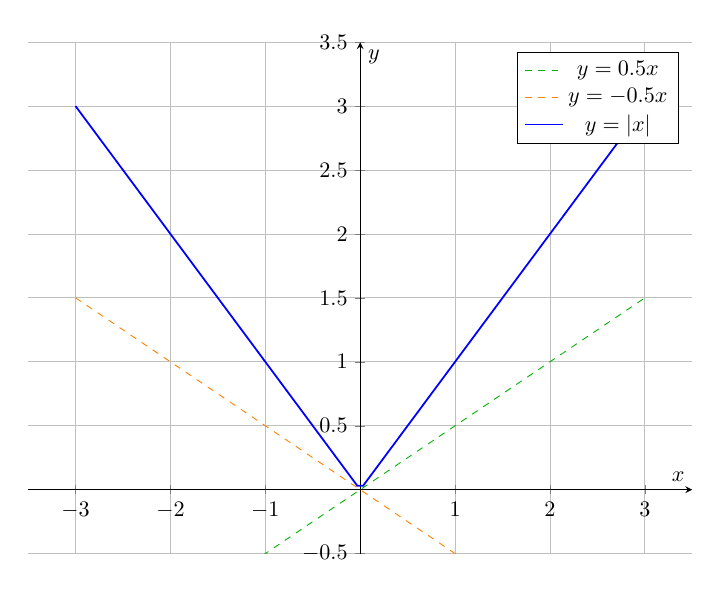
\begin{tikzpicture}[scale=0.8]
          \begin{axis}[
            axis lines=middle,
            xlabel={$x$},
            ylabel={$y$},
            domain=-3:3,
            samples=100,
            ymin=-0.5,
            ymax=3.5,
            xmin=-3.5,
            xmax=3.5,
            width=\textwidth,
            height=0.8\textwidth,
            grid=major,
            ]
            % Lines through origin (strictly below)
            \addplot[green!70!black, dashed, domain=-3:3] {0.5*x};
            \addplot[orange, dashed, domain=-3:3] {-0.5*x};
            % Absolute value function
            \addplot[blue, thick] {abs(x)};
            \legend{$y = 0.5x$, $y = -0.5x$, $y = |x|$}
          \end{axis}
        \end{tikzpicture}
        \caption{Absolute value function with linear bounds}
        \label{fig:absolute}
      \end{subfigure}
      \hfill 
      \begin{subfigure}[b]{0.48\textwidth}
        \centering
        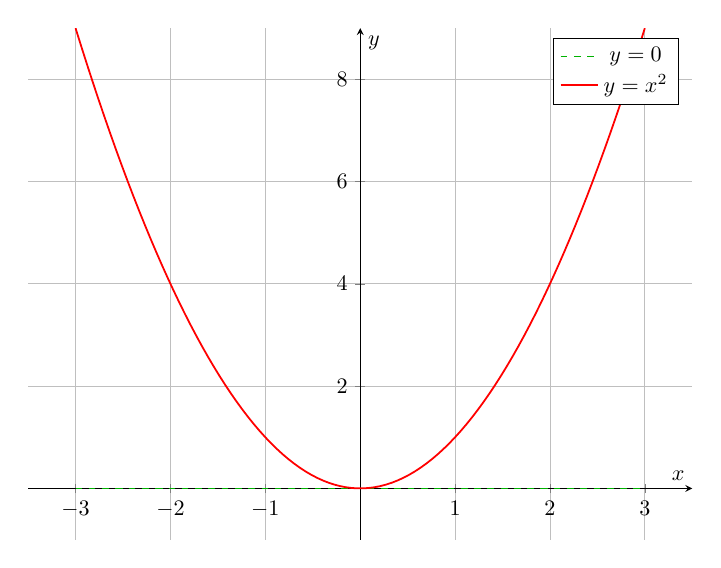
\begin{tikzpicture}[scale=0.8]
          \begin{axis}[
            axis lines=middle,
            xlabel={$x$},
            ylabel={$y$},
            domain=-3:3,
            samples=100,
            ymin=-1,
            ymax=9,
            xmin=-3.5,
            xmax=3.5,
            width=\textwidth,
            height=0.8\textwidth,
            grid=major,
            ]
            % Horizontal line through origin (strictly below)
            \addplot[green!70!black, dashed, domain=-3:3] {0};
            % Quadratic function
            \addplot[red, thick] {x^2};
            \legend{$y = 0$, $y = x^2$}
          \end{axis}
        \end{tikzpicture}
        \caption{Quadratic function with horizontal bound}
        \label{fig:quadratic}
      \end{subfigure}
      \caption{Basic mathematical functions with linear bounds through the origin}
      \label{fig:functions}
    \end{figure}
  \end{definition}

  Note that there can be multiple supporting lines. 

  \begin{theorem}[Jensen's Inequality]
    suppose $\varphi$ is convex on $\mathbb{R}$, with $f, \varphi \circ f$ integrable. Then, 
    \begin{equation}
      \varphi \bigg( \int_0^1 f \,dx \bigg) \leq \int_0^1 \varphi (f(x)) \,dx
    \end{equation}
  \end{theorem}
  \begin{proof}
    This first proof is good intuitively, but not a neat proof.  This is like the definition of convexity, but in a ``continuous  appearance.'' Note that we can think of these as Riemann sums, 
    \begin{equation}
      \varphi \bigg( \sum f_i \Delta x_i \bigg) \leq \sum_{i} \varphi_i \varphi(f_i) \Delta x_i
    \end{equation}
    and then you can pass through the limit to get the integral version. But this is a good intuition. 
  \end{proof}
  \begin{proof}
    The second proof is neater. Set $\alpha = \int_0^1 f\,dx$. Choose $k$ between $\varphi^\prime (\alpha^-), \varphi^\prime (\alpha^+)$. Then, the line 
    \begin{equation}
      \ell(x) \coloneqq k (x - \alpha) + \varphi(\alpha) 
    \end{equation}
    is supporting for $\varphi$, so $\varphi(x) \geq \ell(x)$. Also, $\varphi(f(x)) \geq \ell (f(x))$. Integrate 
    \begin{equation}
      \int_0^1 \varphi (f(x)) \,dx \geq \int_0^1 \Big( \underbrace{k (f(x) - \alpha)}_{= 0} + \varphi(\alpha) \Big) \,dx = \varphi \bigg( \int_0^1 f\,dx \bigg)
    \end{equation}
  \end{proof} 

  On $[a, b]$, we have to normalize $f$, 
  \begin{equation}
    \varphi \bigg( \frac{1}{b - a} \int_a^b f(x) \bigg) \leq \frac{1}{b - a} \int_a^b \varphi (f(x)) \,dx
  \end{equation}

